\chapter{Design Architetturale}

\section{Architettura generale}

Una delle possibili rappresentazioni ad alto livello dell'architettura Client-Server del progetto AmongSus pu\`o essere rappresentato come in Figura \ref{fig:RapArcGen}:

\begin{figure}[ht]
\centering
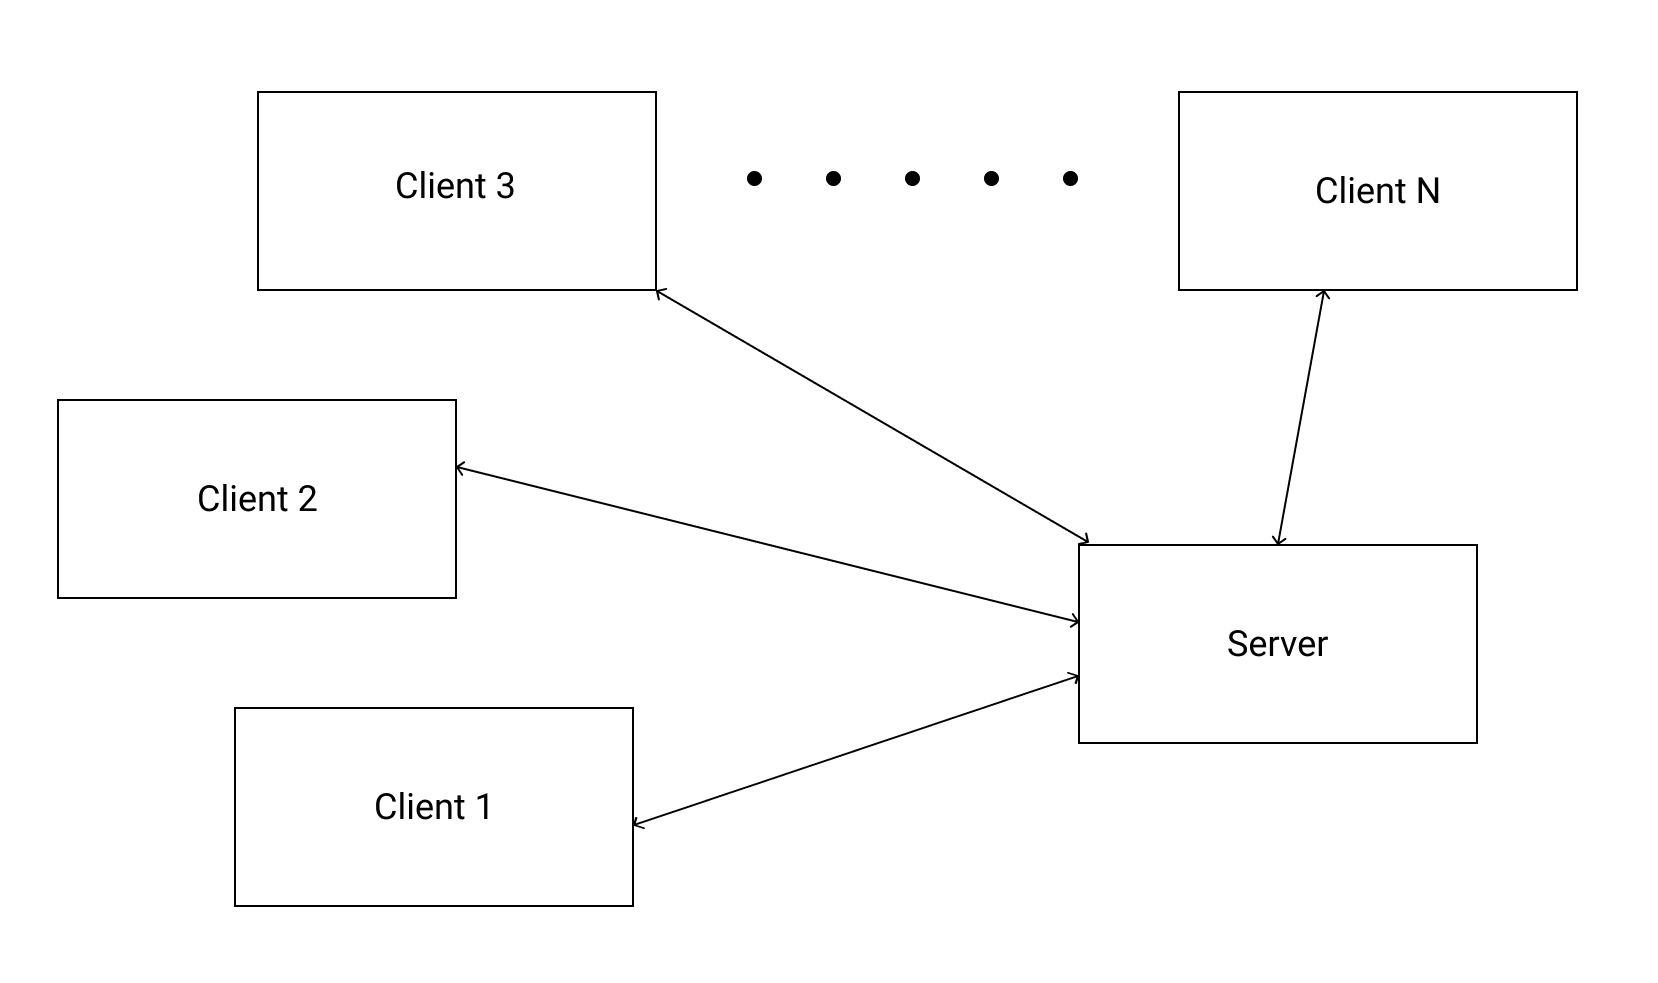
\includegraphics[width=12cm, height=8.5cm]{doc/report/img/ArchitetturaGenerale.png}
\caption{Rappresentazione architettura generale}
\label{fig:RapArcGen}
\end{figure}

Ogni giocatore viene rappresentato da un Client ed un unico Server si occupa della gestione delle connessioni tra giocatori e successivamente dello svolgimento della partita.\\
Questo particolare tipo di architettura \`e stata reputata migliore rispetto a quella Peer-To-Peer. In quest'ultima risulterebbe infatti pi\`u ostico garantire l'autenticit\`a delle connessioni, la loro sincronizzazione e la distribuzione di eventuali informazioni. Nonostante il Peer-To-Peer avrebbe garantito una migliore scalabilit\`a,  si \`e ritenuto più opportuno scegliere l'architettura Client-Server.\\
Tramite quest'architettura si riesce comunque a soddisfare i requisiti non funzionali di scalabilit\`a orizzontale. Oltre a questo si ha un vantaggio sia per quanto riguarda l'aspetto della sicurezza del sistema sia per l'aspetto della semplicit\`a di sviluppo.\\

\subsection{Core}
Descrive unicamente, in maniera indipendente dagli altri moduli, la definizione delle entit\`a base e delle regole che caratterizzano il gioco Among Us.\\
Espone delle API che possono essere utilizzate dai vari moduli dell'applicazione che dipendono da esso. Per tale ragione il Core può essere considerato come una vera e propria libreria esterna che non conserva alcuno stato relativo allo svolgimento del gioco.\\
In particolare, il Server lo utilizza per l'aggiornamento della partita in risposta alle mosse degli altri giocatori e il controllo della condizione di vittoria. \\
Il Client lo utilizza per la gestione interna del gioco, ovvero la validazione dei movimenti, le azioni dei giocatori nella schermata e per le interazioni con il Server relative agli aggiornamenti della schermata di gioco.

\subsection{Server}
Il Server \`e stato diviso in più componenti, i principali sono:
\begin{itemize}
    \item \textbf{LobbyManagerActor}: Si occupa  della gestione delle connessioni dei Client alle \textit{lobby}. In particolare ha il compito di creare \textit{lobby} pubbliche o private. Una volta raggiunto un numero sufficiente di partecipanti, genera un \textit{GameManagerActor} che da quel momento in poi si occupa della gestione del gioco.
    \item \textbf{GameManagerActor}: Viene creato e richiamato per occuparsi della partita in corso. Quando il sistema \`e in fase di runtime, verranno creati molteplici attori di \textit{GameManager}, uno per ogni \textit{lobby}. Esso si occupa di ricevere le varie attivit\`a dei partecipanti e di aggiornare quelli presenti dei cambiamenti della partita come, ad esempio, \textit{Kill} e \textit{Emergency}.
\end{itemize}

\subsection{Client}
Per la realizzazione del Client è stato utilizzato il modello ad Attori cercando di rispettare il pattern MVC. La soluzione \`e stata organizzata per meglio isolare e suddividere i vari compiti:
\begin{itemize}
    \item \textbf{Model}: Si occupa della gestione dei dati, della logica e mantiene lo stato del gioco.\\
    Comunica tramite il \textit{ModelActor} con il \textit{ControllerActor} notificando i propri cambiamenti interni e ricevendo gli aggiornamenti degli altri Client.
    \item \textbf{View}: Gestisce la user interface durante tutte le fasi del gioco, aggiornandosi a seguito di input dell'utente e/o cambiamenti del model.\\
    La comunicazione avviene grazie allo scambio di messaggi tra il proprio attore \textit{UiActor} e l'attore del Controller \textit{ControllerActor}.
    \item \textbf{Controller}: Il Controller ha il compito di avviare l'applicazione ed istanziare il \textit{ControllerActor} che deve sucessivamente svolgere le seguenti attività:
    \begin{itemize}
        \item Connessione con il server;
        \item Gestione dei messaggi tra gli attori.
        \item Gestione della fase di lobby;
        \item Gestione della fase di gioco;
        \item Gestione dei Timer per le azioni a tempo del gioco;
        \item Gestione della fase di votazione;
        \item Gestione della fine della partita.
    \end{itemize}
\end{itemize}

\subsection{Architettura ad Attori}
Durante la fase di analisi e pianificazione dell'applicazione, si \`e notato subito il bisogno di uno scambio quasi continuo di informazioni/messaggi tra le varie entit\`a della architettura.\\
Per questo motivo si \`e optato per l'utilizzo di un modello ad Attori (vedi Figura \ref{fig:RapConcDeAct}), sfruttando il Framework \textbf{Akka}.\\
Questo modello permette di modellare problemi altamente concorrenti attraverso un modello a scambio di messaggi asincrono. La modellazione ad attori, grazie alla proprietà di isolamento tra enti computazionali distinti, e grazie ad una solida organizzazione gerarchica delle responsabilità, pemette di ragionare in maniera semplificata su problemi nei quali la concorrenza, distribuzione e gestione dei failure sarebbero altrimenti molto difficili da trattare.\\

\begin{figure}[ht]
\centering
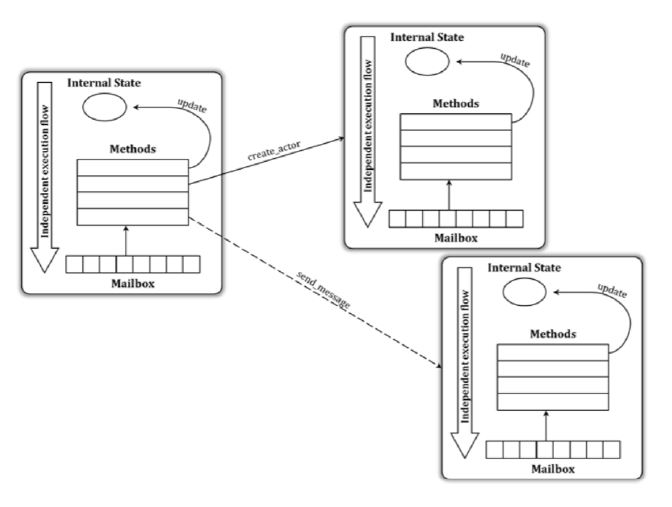
\includegraphics[width=\textwidth, scale=0.44]{img/Actor.jpg}
\caption{Rappresentazione concettuale degli Attori}
\label{fig:RapConcDeAct}
\end{figure}

Un Attore \`e un'entit\`a autonoma che possiede un proprio flusso di controllo ed è caratterizzato da:
\begin{itemize}
    \item \textbf{Nome}: Permette di riconoscere univocamente l'attore all'interno del sistema;
    \item \textbf{Immutabilit\`a dello Stato Interno}: Lo stato interno degli attori \`e immutabile ed il cambiamento viene espresso tramite cambio di Behaviour;
    \item \textbf{Behaviour}: Permette di utilizzare l'Attore come se fosse una macchina a stati finiti che reagisce agli input, ovvero i messaggi, ricevuti;
\end{itemize}
L'Attore ha la possibilit\`a di comunicare il risultato delle sue operazioni in tre differenti modi:
\begin{itemize}
    \item Aggiornamento del proprio stato interno;
    \item Invio di uno o pi\`u messaggi ad un altro Attore;
    \item Creazione di un nuovo Attore;
\end{itemize}

\subsubsection{Utilizzo Architettura ad Attori}
Sfruttando il paradigma ad attori ci si è potuto concentrare sulle interazioni tra le entit\'a e studiare un'architettura che ottimizzasse le comunicazioni e lo scambio di informazioni. L'architettura derivante dall'applicazione di tale modello al nostro sistema ha portato a quella mostrata in Figura \ref{fig:ArchSisAct}.

\begin{figure}[ht]
\centering
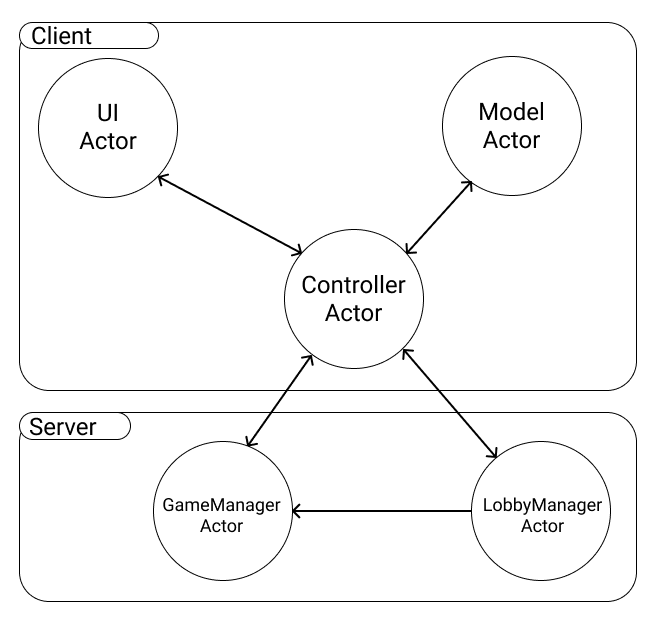
\includegraphics[width=11cm, height=10.5cm]{img/ActorScheme.png}
\caption{Architettura del Sistema Basata su Attori}
\label{fig:ArchSisAct}
\end{figure}

\subsubsection{Comunicazione Client}
\begin{itemize}
    \item \textbf{ControllerActor}: Riceve le azioni compiute dall'utente tramite lo \textit{UiActor}, comunica tutti i cambiamenti del gioco al \textit{ModelActor}. Viceversa riceve notifiche riguardanti il cambiamento di stato del \textit{ModelActor} e le inoltra allo \textit{UiActor};
    \item \textbf{UiActor}: Notifica il Controller delle azioni compiute dall'utente sull'interfaccia grafica, riceve notifiche dal \textit{ControllerActor} e visualizza i cambiamenti nel Frame corrente;
    \item \textbf{ModelActor}: Riceve i messaggi che richiedono l'aggiornamento/modifica del proprio stato, effettua l'aggiornamento del proprio stato e lo notifica al \textit{ControllerActor};
\end{itemize}

\subsubsection{Comunicazione Client-Server}
\begin{itemize}
    \item \textbf{ControllerActor}: Si occupa inoltre della comunicazione con il Server. In particolare notificando, ricevendo ed aggiornando lo stato del gioco al \textit{GameManagerActor} o della \textit{lobby} al \textit{LobbyManagerActor};
    \item \textbf{LobbyManagerActor}: Invia e riceve messaggi dal ControllerActor riguardo la gestione della \textit{lobby};
    \item \textbf{GameManagerActor}: Ha il compito di inviare e ricevere messaggi dal \textit{ControllerActor} riguardo la gestione e l'aggiornamento dello stato del gioco tra i vari giocatori;
\end{itemize}
\`E stata fatta questa scelta per riuscire a garantire prestazioni ottimali durante l'esecuzione del gioco.
Inoltre il sistema \`e stato modellato in maniera tale da prevedere modifiche future.